
\subsection{Realistic High-Frequency Ground Motion}

\textcolor{red}{Pending contribution to be asked of Kim Olsen. It should focus on how UCVM small-scale heterogeneities generator is helping advance ground motion simulations toward a more realistic representation of high-frequency shaking characteristics. We suggest this section be accompanied with an image such as that shown in Figure \ref{fig:heterogeneities} which compares ground motion with and without small scale heterogeneities.}

\ \ \ %This is a little trick to avoid problems with PDF compilation.  We can erase this line later.

\ \ \ %This is a little trick to avoid problems with PDF compilation.  We can erase this line later.

\begin{figure*}[ht!]
    \centering
    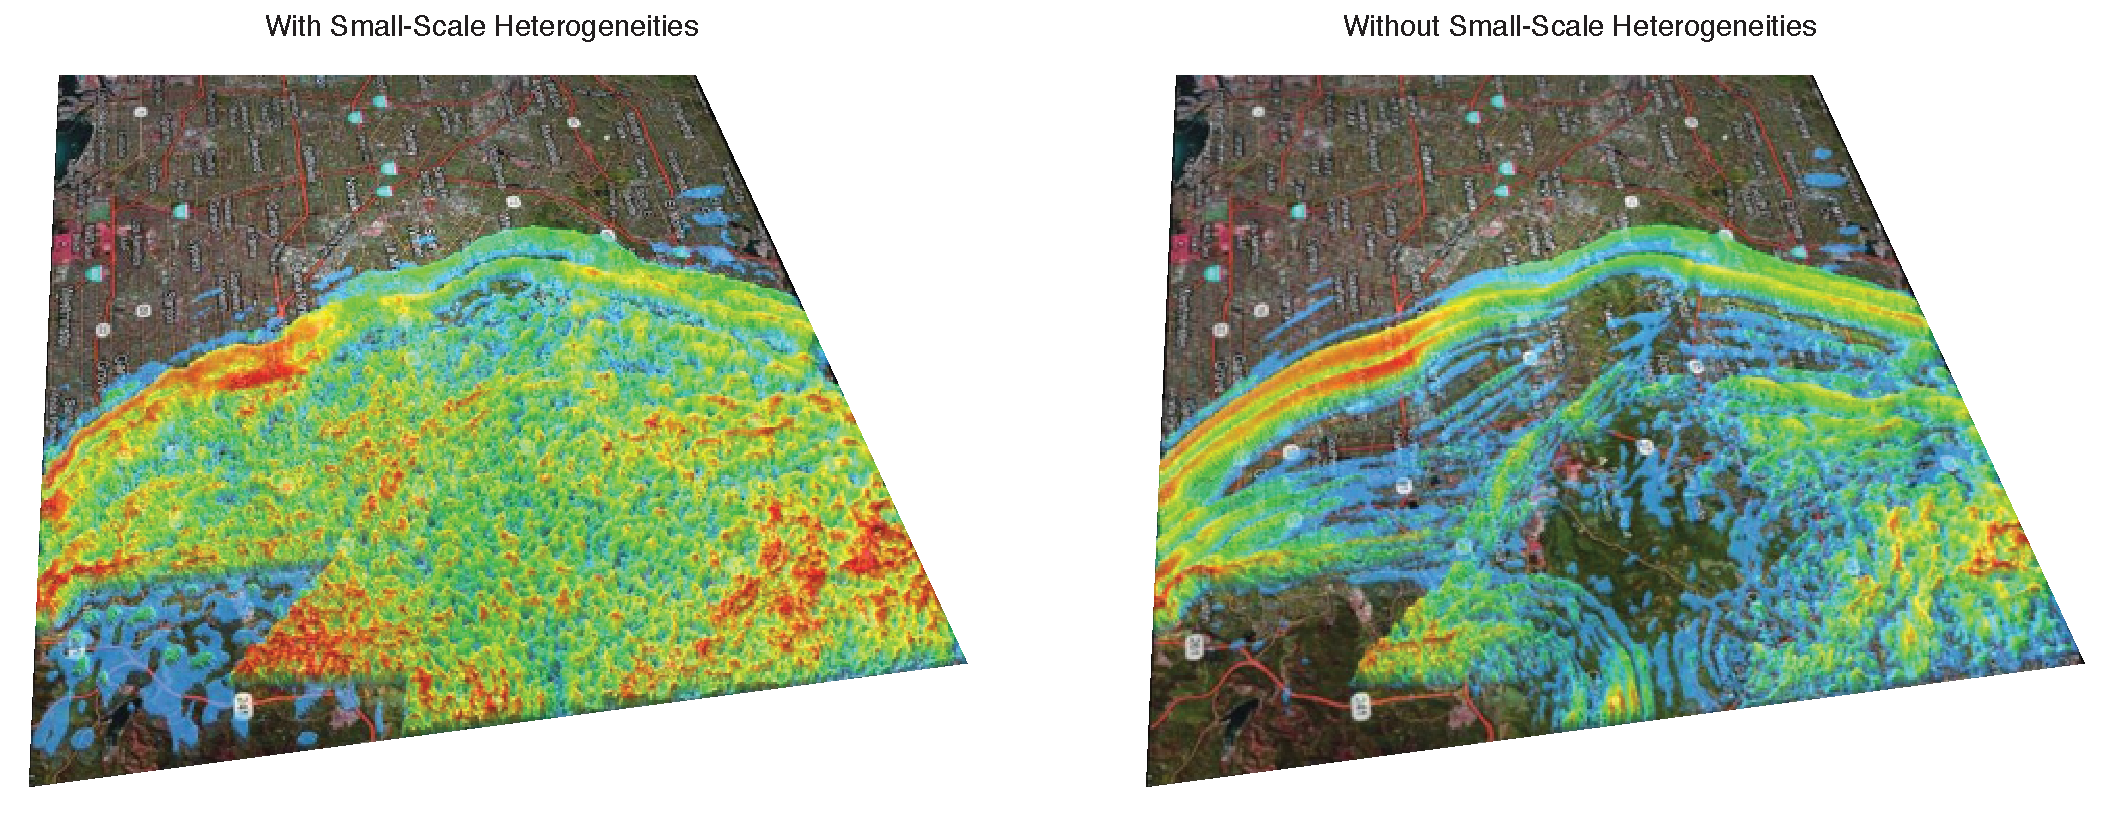
\includegraphics
        [width=0.80\textwidth]
        {figures/pdf/heterogeneities}
    \caption{\textcolor{red}{Comparison of two simulation results with and without considering the effects of small-scale material heterogeneities. The images show still-frames of the velocity magnitude at the earth's surface for the 29 July 2008, \eqmag{w} 5.4 Chino Hills, California earthquake. The underlying models used for these simulations were built using the UCVM meshing and small-scale heterogeneities utilities.}}
    \label{fig:heterogeneities}
\end{figure*}

